% !TEX root = ../main.tex
% --+ Strong Coupling Constant +------------------------------------------------
\subsubsection{Strong Coupling Constant $\alpha_s$}
    Measuring the experimental value of $\alpha_s$ is important for perturbative QCD calculations.
    To do this, one should determine the overall scale of renormalisation.
    This is usually selected to be the mass of the neutral Bose particle $Z^0$, which is $91.19$ GeV.
    Additionally, one should fix the scheme of renormalisation, which defines the coupling constant in a given scale.
    The experimental results for $\alpha_s$ can be seen on figure

    \begin{figure}[b!] % NOTE. Figure out source.
        \centering\frame{
        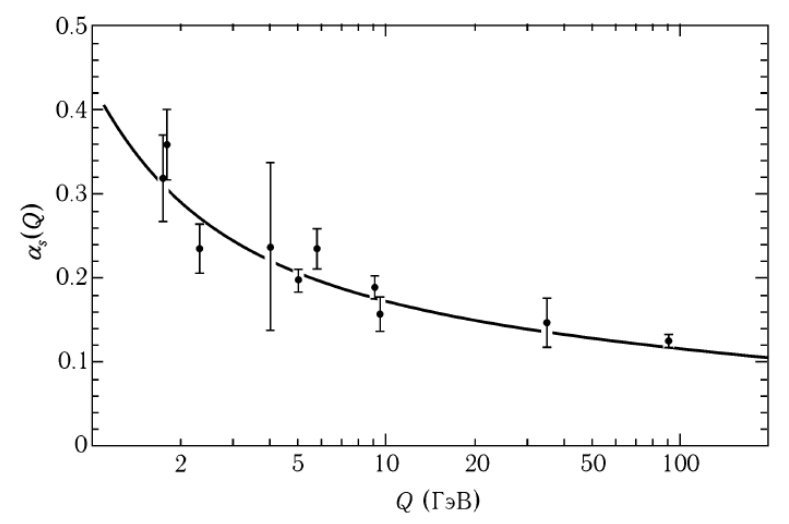
\includegraphics[width=0.8\textwidth]{10physicsmotivation/img/11strong_coupling_constant_q.png}}
        \caption[$\alpha_s$ dependence on $Q^2$.]{Experimentally measured $\alpha_s$ dependence on $Q$.
        The measured values are compared with theoretical predictions of renormalised evolution with initial $\alpha_s(m_z) = 0.117$ GeV.}
        \label{fig::alpha_q_dependence}
    \end{figure}
